\newpage
\section{Introduction}

\subsection{Laser Locking}

The ability to lock a laser to a very specific frequency is of great importance to the UBC Quantum Degenerate Gases Laboratory.  They use these optical systems to laser cool atomic and molecular gases.  This requires a very narrow linewidth on the laser, and a specific frequency.  Any improvement in the frequency precision of the laser will increase the quantity of atoms that can be trapped or cooled, as well as the attainable temperatures in a trap.  Often, this frequency must be very close to the natural transitions of the gas.

One way to acquire such a system is to pass the beam through a gas.  The gas has several transitions at certain energies, which can be detected by sweeping the laser (or an associated probe beam).  When doing this, the gas atoms will absorb energies at the corresponding frequencies, which will appear on a spectrum analyser.  However, since the gas is at room temperature, the dip will have a bandwidth of about 1GHz, which is too wide to lock a laser to.

\subsection{Doppler Effects}

Since the gas atoms are moving in different directions, some atoms will be moving towards the laser beam, and other atoms will be moving away from the laser (some will be in between, of course).  As a result, if we use a single laser, the atoms moving towards the laser will perceive a higher frequency, and thus will excite at lower frequencies than the resonance frequency.  The opposite is also true.  If we measure the absorption-vs-frequency curve for a laser passed through the gas, we get a wide smear that is approximately 1GHz wide \cite{madison14}.

This makes the apparent spectrum of the gas much wider, and thus, much harder to lock a signal to.

A major improvement is to redirect the single frequency laser around the sample, to the opposite side.  Now, when the sweep laser is at the same frequency as the pumping laser, its light will not be absorbed by the atoms with zero horizontal velocity.  This creates a Doppler-cancelled feature, which is much narrower in bandwidth.

\begin{figure}
    \centering
    \label{fig:doppler}
    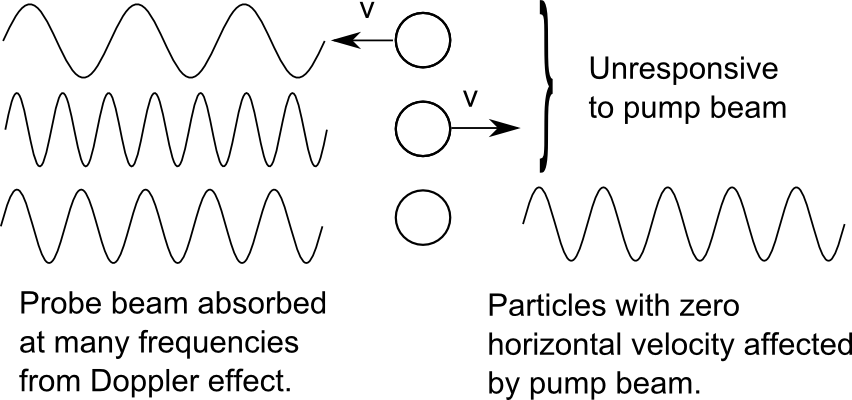
\includegraphics{doppler.pdf}
    \caption{Doppler effect demonstration.  Probe beam is absorbed across a wide frequency range, but only the non-Doppler-shifted particles are affected by both beams from left and right.}
\end{figure}

\subsection{Acousto-Optic Modulator}

One way to modulate the frequency of the beam is to use an *acousto-optic modulator* (AOM).  An AOM is a device that acoustically varies its shape, adjusting the distance the light has to travel to reach its destination.  By modulating this at a frequency $\Omega$, we produce a beam of light with sidebands at $\omega + \Omega$ and $\omega - \Omega$, where $\omega$ is the original frequency of the laser.

Since these devices use acoustics, they are limited by the mechanical properties of the device.  As a result, the AOM in use by the sponsor has a maximum frequency of about 100kHz.

\subsection{Electro-Optic Modulator}

An \emph{electro-optic modulator} (EOM), is a device that uses an electric field to modulate the phase of a light wave.  These typically take advantage of the \emph{Pockels effect}, whereby the speed of light in a crystal is affected by the presence of an electric field.  Therefore, by adjusting the electric field in the crystal, the phase (and ultimately frequency spectrum) of the beam can be adjusted.

Unfortunately, the Pockels effect requires very large voltages to operate, on the order of hundreds of volts.  Some manufacturers provide a full EOM solution, with built-in amplifier, to make their equipment easier to use, making an external high-voltage amplifier unnecessary.


